\documentclass[12pt,a4paper]{article}
\usepackage{vmargin}
\setmarginsrb{1.0in}{1.0in}{1.0in}{1.0in}{0mm}{0mm}{0mm}{10mm}

\usepackage{amsfonts,amsmath,amssymb}
\usepackage{amsthm}
\usepackage{graphicx}
\usepackage{amsmath}
\usepackage{xcolor}
%\usepackage{ngerman}
\usepackage{listings}
\usepackage[utf8]{inputenc}
%\usepackage[T1]{fontenc}
\usepackage{comment}
\usepackage{algorithm}
\usepackage{hyperref}
%%\usepackage{algpseudocode}
\renewcommand*\thealgorithm{}
\usepackage{algorithmic}
\usepackage{amsmath}

\newcommand{\N}{\mathbb{N}}
\newcommand{\R}{\mathbb{R}}
\renewcommand{\O}{\mathcal{O}}
\usepackage{mathtools}

\newtheorem{theorem}{Theorem}
\newtheorem{lemma}{Lemma}
\newtheorem{corollary}[theorem]{Corollary}
\newtheorem{conjecture}{Conjecture}
\newtheorem{fact}[theorem]{Fact}
%\newtheorem{proposition}[theorem]{Proposition}
\newtheorem{observation}{Observation}
%\newtheorem{notation}[theorem]{Notation}
\newtheorem{remark}{Remark}
\newtheorem{claim}{Claim}
\newtheorem{definition}{Definition}
%\theoremstyle{definition}
%\newtheorem{problem}[theorem]{Problem}
\newtheorem{example}{Example}
%\renewcommand{\qedsymbol}{\rule{1mm}{1mm}}
\newcommand\independent{\protect\mathpalette{\protect\independenT}{\perp}}
\renewcommand{\thesubsection}{\thesection.\alph{subsection}}
%\def\thesection{\alph{section}}
\setcounter{section}{1}

\setlength{\parindent}{0pt}


\begin{document}

\noindent
\begin{minipage}{0.66\textwidth}
Hasso Plattner Institute Potsdam\\
\\
Seminar on Nature Inspired Algorithms\\ Summer 2017\\
Potsdam, \today
\end{minipage}
~
\begin{minipage}{0.30\textwidth}

\includegraphics[width=\textwidth]{../homework_template/Hasso_Plattner_Institut_Logo}
\end{minipage}


\begin{center}
 {\LARGE \textbf{Homework 2}}
 \vspace*{0.5cm}\\
 {\SMALL \text{Willi Gierke}}
\end{center}
%%%%%%%%%%%%%%%%%%%%%%%%%%%%%%%%%%%%%%%%%%%


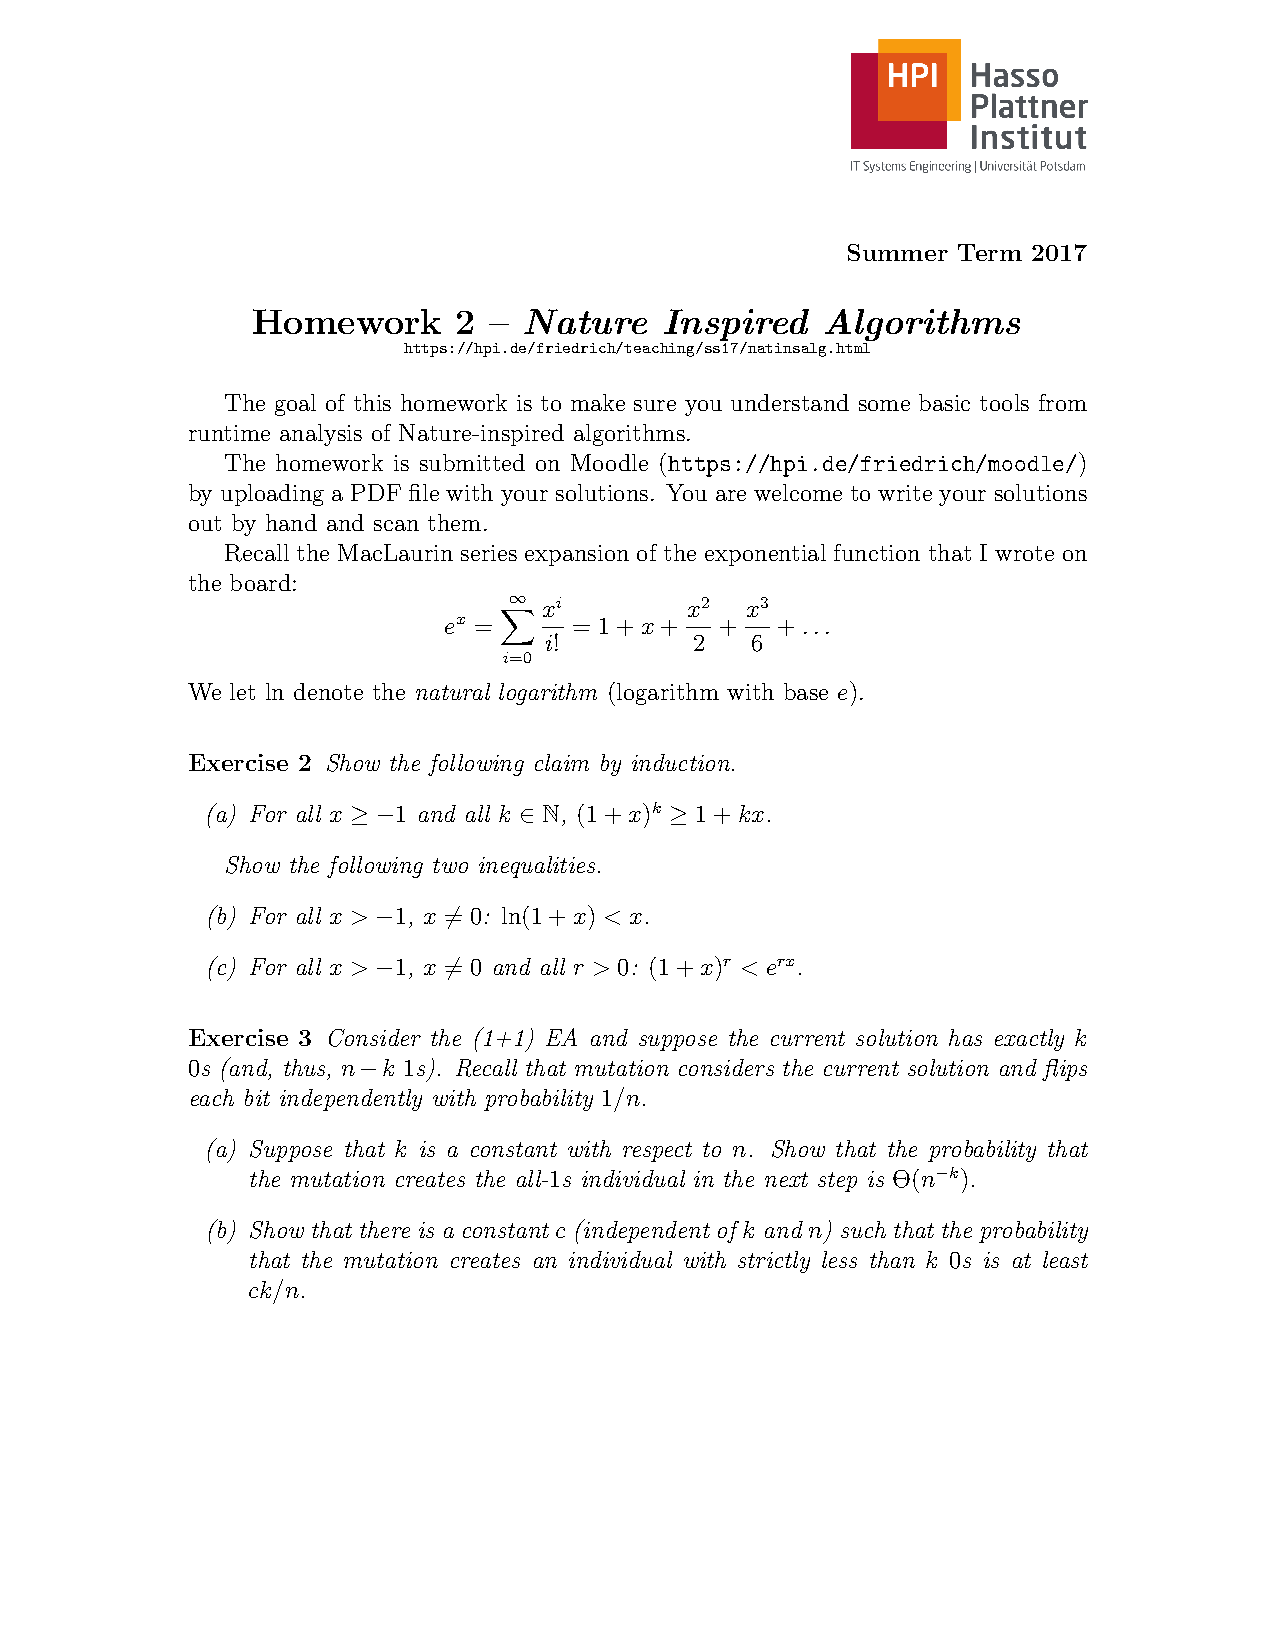
\includegraphics[clip, trim=0.5cm 2.5cm 0.5cm 4cm, width=0.99\textwidth]{homework02.pdf}
\clearpage

\section{Exercise}
\subsection{}
\begin{claim}
For all x $\geq-1$ and all k \in \mathbb{N}: (1 + x)^k \geq 1 + kx
\end{claim}

\begin{proof}
\\Base case $k=1$: $(1 + x)^1 \geq 1 + 1 \cdot x$

Inductive hypothesis: Suppose the theorem holds for all values of $k$ up to some $n$, $n \geq 1$.
Inductive step: Let $k=n+1$
\begin{align}
  (1 + x)^n & \geq 1 + nx && \cdot (1 + x)\\
  (1 + x)^{n+1} & \geq (1 + nx)(1+x) \\
  (1 + x)^{n+1} & \geq 1 + x + nx + nx^2 \\
  (1 + x)^{n+1} & \geq 1 + (n+1)x + nx^2 \\
  (1 + x)^{n+1} & \geq 1 + (n+1)x + nx^2 \geq 1 + (n+1)x && \text{since } nx^2 \geq 0\\
  (1 + x)^{n+1} & \geq 1 + (n+1)x \\
\end{align}
So the theorem holds for $k=n+1$.
By the principle of mathematical induction, the theorem holds for all $k \in \mathbb{N}$.
\end{proof}

\subsection{}
\begin{claim}
For all x $>-1$, x \neq 0: \ln(1+x) < x
\end{claim}

\begin{proof}
The idea is to proof that $f(x)=\ln(1+x)-x$ is negative for all x $>-1$, x \neq 0. \\

\begin{align}
  f'(x) &= \frac{1}{1+x}-1 \\
  0 &= \frac{1}{1+x_E}-1 && \cdot (x_E + 1) \\
  0 &= x_E \\
  f''(x_E) &= -\frac{1}{(1+x_E)^2} < 0 \rightarrow \text{P(0\textbar 0) is local maximum}\\
\end{align}
This shows that $f(x)$ is only non-negative at its single global maximum P(0\textbar 0) but negative otherwise.
Since the theorem is not supposed to hold for $x=0$ it is proven.
\end{proof}

\clearpage

\subsection{}
\begin{claim}
For all x $>-1, x \neq 0$ and all $r > 0: (1+x)^r < e^{rx}$
\end{claim}

\begin{proof}
\begin{align}
  (1+x)^r &< e^{rx} && \ln \text{ since } x \neq 0\\
  \ln((1+x)^r) &< \ln(e^{rx}) && \text{Logarithm power rule}\\
  r \cdot \ln(1+x) &< rx && \text{: $r$ since } r \neq 0\\
  \ln(1+x) &< x && \text{See Claim 2}
\end{align}
\end{proof}


\section{Exercise}
\subsection{}
\begin{proof}

\begin{align}
  P(X=n) &= \left(\frac{1}{n}\right)^{k}\left(1-\frac{1}{n}\right)^{n-k} \\
  &= n^{-k}\left(1-\frac{1}{n}\right)^{n}\left(1-\frac{1}{n}\right)^{-k} && \lim_{n \to \infty} \\
  &= n^{-k} && \text{since } \left(1-\frac{1}{n}\right)^{n} = 1 \text{ and }\left(1-\frac{1}{n}\right)^{-k}=1 \\
  &= \Theta(n^{-k})
\end{align}

\end{proof}

\subsection{}
\begin{proof}
\begin{align}
  P \text{("Flip 1\ldots k 0's")} & \geq P \text{("Flip k 0's")} = \frac{k}{n}\left(1-\frac{1}{n}\right)^{n-k} \geq \frac{k}{en} \\
  & \geq c\frac{k}{n} \text{ for } c = \frac{1}{e}
\end{align}

\end{proof}

\end{document}
